%========================================================================================
% TU Dortmund, Informatik Lehrstuhl VII
%========================================================================================

\chapter{Anwendung des Spring-Embedders auf den modellierten Graphen}
\label{Kapitel 4}
%

Der in Kapitel 3 vorgestellte Algorithmus wird nun so erweitert und angepasst, dass er für den gegebenen Graphen und unser Problem passend ist. Das Ziel wird es sein, den aus Kapitel 2 gewonnen Graphen mithilfe des Algorithmus zu einer MetroMap ähnlichen Darstellung zu führen. Die besonders leichte Erweiterbarkeit und Modifizierbarkeit des Algorithmus erlauben dies und ist auch der Grund, weshalb dieser Algorithmus als Basis zur Lösung des Problems verwendet wurde. \\

Das Erstellen dieses Layouts im Vergleich zur herkömmlichen MetroMap unterscheidet sich vor allem durch:

\begin{itemize}
	\item eine deutlich striktere Beibehaltung der topologischen und geographischen Eigenschaft des Graphen
	\item das Verteilen der Knoten auf die komplette Oberfläche soll nicht stattfinden
	\item es existieren Knoten, die sich nicht bewegen lassen
	\item durch das modellieren der Leiterseile existiert eine bestimmte Struktur innerhalb des Graphen, die noch immer sichtbar bleiben soll
	\item nichts außerhalb des Platzierens von Knoten und Kanten wird angewendet, das sind vor allem, bei einer MetroMap, das Erstellen von Labels und die Färbung von Kanten.
\end{itemize} 

Der vorgestellte Algorithmus in Kapitel 3 wandelt einen Graphen ebenso nicht in eine perfekte MetroMap um. Orthogonalität wird komplett ignoriert. Durch das zufällige Platzieren der Knoten, wird jegliche Topologie des Graphen entfernt und alle anderen ausmachenden Komponenten einer MetroMap werden nicht erstellt. Ausschließlich das Platzieren der Knoten und Kanten sind beim Erstellen des neuen Layouts von Bedeutung, dh. es wird bei der Platzierung auch nicht auf mögliche Positionen der Labels geachtet. Das Ziel ist es demnach nun den Algorithmus den neuen Ansprüchen anzupassen und ein ansprechendes Layout des Ausschnittes des Höchstspannungsnetzes zu erstellen. Dieser Ausschnitt  kann anschließend beliebig erweitert werden oder das komplette Höchstspannungsnetz umfassen.  


\section{Nachteile des Spring-Embedders auf der Anwendung des Graphen}
\label{Kapitel_4_-_Unterkapitel_2}

\begin{figure}[t]
	\centering
	{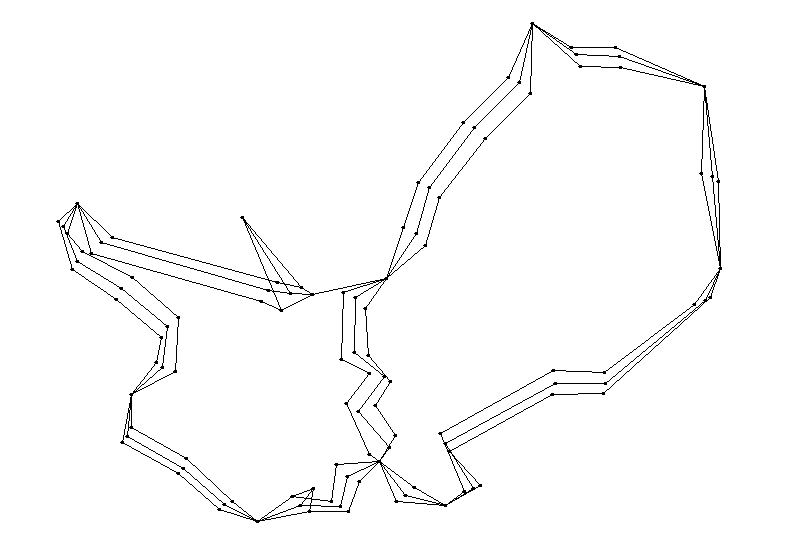
\includegraphics[scale=0.8]{bilder/graph10iterationenreingold}\label{fig_dortmundmap}
	}\\
	\caption[Dortmunder MetroMap]{Dortmunder MetroMap [http://www.urbanrail.net/eu/de/do/dortmund-map.png]}
	\label{fig_dortmundmap}
\end{figure}
\begin{figure}[t]
	\centering
	{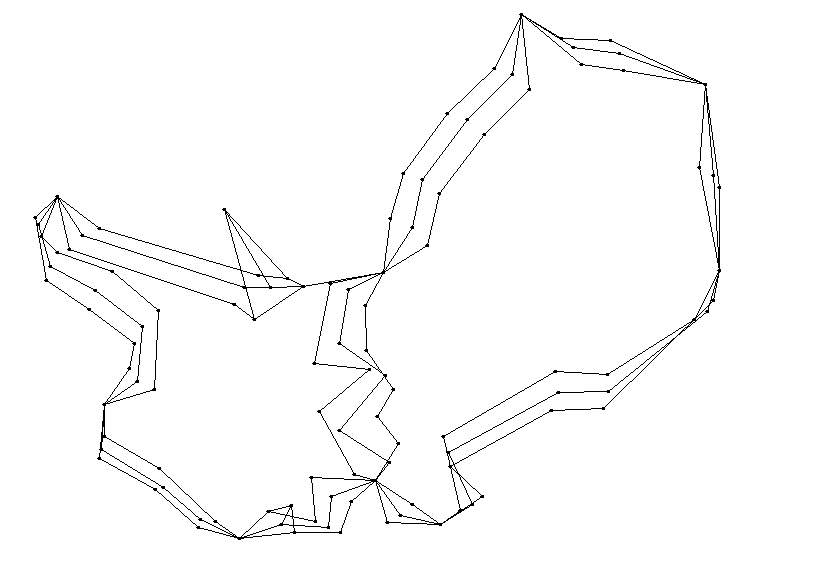
\includegraphics[scale=0.8]{bilder/graph25iterationenreingold}\label{fig_dortmundmap}
	}\\
	\caption[Dortmunder MetroMap]{Dortmunder MetroMap [http://www.urbanrail.net/eu/de/do/dortmund-map.png]}
	\label{fig_dortmundmap}
\end{figure}
\begin{figure}[t]
	\centering
	{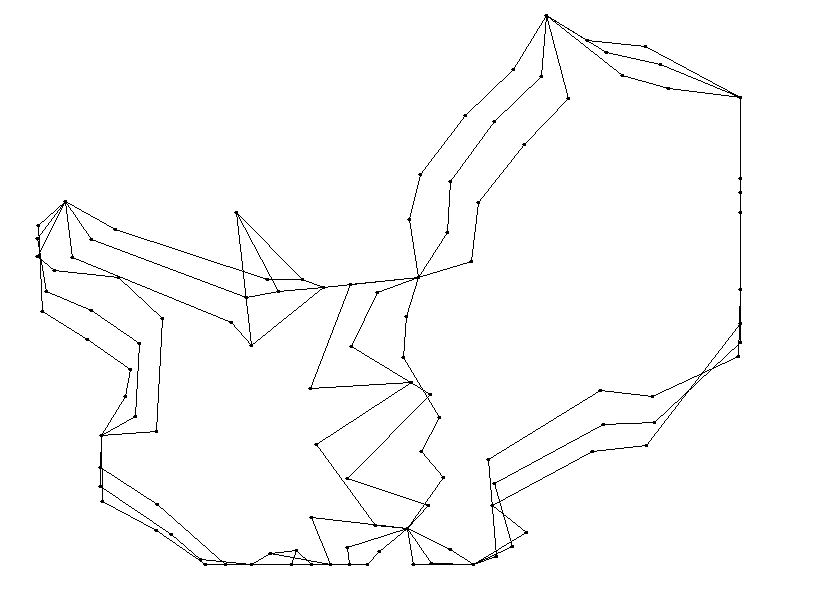
\includegraphics[scale=0.8]{bilder/graph50iterationenreingold}\label{fig_dortmundmap}
	}\\
	\caption[Dortmunder MetroMap]{Dortmunder MetroMap [http://www.urbanrail.net/eu/de/do/dortmund-map.png]}
	\label{fig_dortmundmap}
\end{figure}
Im Folgenden wird der Algorithmus unmodifiziert auf den Graphen angewendet um deutlich zu machen, wo die grundsätzlichen Probleme dieses Algorithmus liegen und was verbessert werden muss. Dazu wird dieser mit einer verschiedenen Anzahl an Iterationen auf den Graphen angewendet und anschließend ausgewertet. Existierten keine Bewegungseinschränkungen für die Knoten und würde der Algorithmus so auf den Graphen angewendet werden, würden viele unerwünschte Nebeneffekte eintreten, die den Graphen noch unästhetischer machen. In den Abbildung 4.1/2/3 wird der resultierende Graph dargestellt nach jeweils 10, 25 und 50 Iterationen.\\

Nach 10 Iterationen des Algorithmus wird eine deutliche Verbesserung der Abstände der Knoten sichtbar. Das resultiert aus der abstoßenden Kraft der Knoten zueinander. Jedoch treten bei 10 Iterationen schon große Probleme mit der Überschneidung von Kanten auf, was eine nicht planare Darstellung des Graphen zur Folge hat. Dies sollte jedoch unter allen Umständen vermieden werden, denn wie es auf der Abbildung 4.1 schon leicht zu sehen ist, wird durch das Überschneiden von Knoten der Graph sehr unübersichtlich und es wird schwer zu sagen, zu welcher Kante welcher Knoten gehört. Da die vergrößerten Abstände der Knoten auf den langen Verbindungen zu einer deutlichen Verbesserung der Ästhetik führen, sieht der resultierende Graph nach 10 Iterationen, trotz der leichten Überschneidung von Kanten, schon deutlich übersichtlicher aus. \\

Nach weiteren Iterationen des Algorithmus wird die Darstellung zunehmend schlechter und es kommt zu etlichen Überschneidungen der Kanten. Die Knoten stoßen sich weiter ab und sie fangen an sich an die Grenzen der Oberfläche zu bewegen, welches auf der Abbildung 4.2 nach 25 Iterationen am linken, rechten und unteren Rand gut zu sehen ist. Die Knoten fangen an sich dort zu sammeln und trotz ihrer abstoßenden Kraft zueinander wird das Sammeln zunehmend schlimmer. Der ursprüngliche Graph, welcher aus dem Höchstspannungsnetz modelliert wurde, ist noch immer wiederzuerkennen. Die beiden markanten großen Flächen innerhalb des Graphen, welche der ursprüngliche Graph auch besaß, sind noch deutlich zu erkennen. Der Zweck des Algorithmus die Knoten gleichmäßig zu verteilen mit einer optimalen Distanz zu einander wird langsam deutlich durch die größeren Abstände der Knoten. \\

Nach 50 Iterationen, welches auf Abbildug 4.3 zu sehen ist, sind fast alle Knoten bereits deutlich von ihrer Startpositionen bewegt worden. Ursprüngliche Muster, Merkmale oder die Wiedererkennbarkeit dieser Zeichnung im Vergleich des Graphen vor Anwendung des Algorithmus, wird immer schwerer. Die äußeren Grenzen sind sehr deutlich am Rande der Oberfläche zu sehen. Die Knoten sammeln sich dort, da sie sich nicht weiter nach außen entfernen können. Die anderen Knoten fangen an sich in den beiden offenen Flächen des Graphen zu verteilen und zu Positionieren. Es scheint als wäre die Oberfläche nicht groß genug für den Algorithmus mit der gegebenen Anzahl an Knoten, doch auch eine deutliche Verringerung der Knoten führt zum selben Ergebnis, da die optimale Distanz zwischen zwei Knoten noch deutlich zu groß ist. Die Knoten versuchen sich ausnahmslos auf der Oberfläche mit perfekten Abständen zu einander zu verteilen. Dieser Vorgang ist jedoch nicht gewollt, nicht bei dem Layout unseres Graphen noch bei einer grundsätzlichen MetroMap. Es gibt auch sehr viele Ausreißer, die ein lokales Minima nicht mehr überwinden können. Das bedeutet, der Algorithmus wird niemals, eine erst schlechtere Positionierung wählen um anschließend eine bessere zu bekommen. Er wird stets versuchen von Iteration nach Iteration eine bessere Positionierung anhand der Kräfte zu erhalten, auch wenn dies zur Folge hat, dass die Knoten sich möglicherweise nicht optimal Positionieren. \\


\section{Anpassung des Spring-Embedders zur Anwendung auf das modellierte Höchstspannungsnetz}
\label{Kapitel_4_-_Unterkapitel_3}

\begin{figure}[t]
	\centering
	{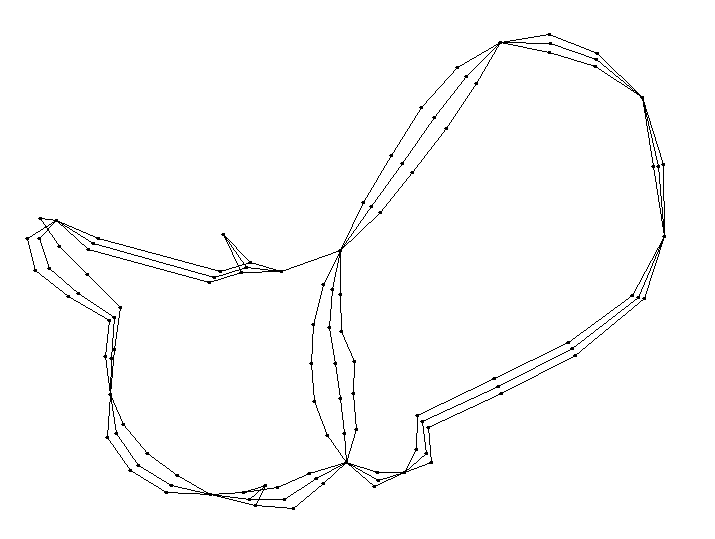
\includegraphics[scale=0.8]{bilder/graph25iterationenreingoldmodified1}\label{fig_dortmundmap}
	}\\
	\caption[Dortmunder MetroMap]{Dortmunder MetroMap [http://www.urbanrail.net/eu/de/do/dortmund-map.png]}
	\label{fig_dortmundmap}
\end{figure}
\begin{figure}[t]
	\centering
	{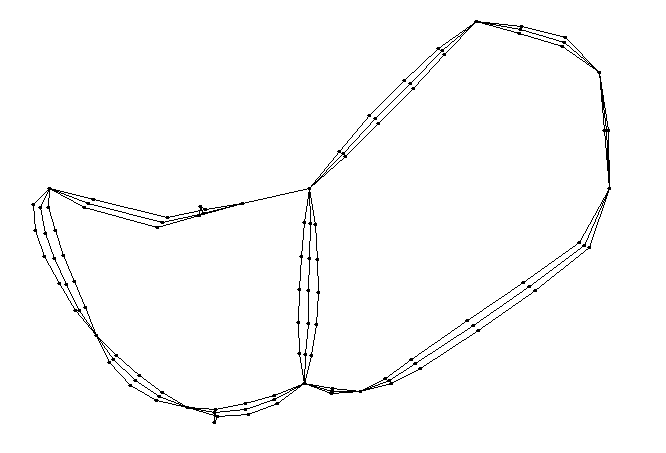
\includegraphics[scale=0.8]{bilder/graph50iterationenreingoldmodified1}\label{fig_dortmundmap}
	}\\
	\caption[Dortmunder MetroMap]{Dortmunder MetroMap [http://www.urbanrail.net/eu/de/do/dortmund-map.png]}
	\label{fig_dortmundmap}
\end{figure}

Zum Anwenden auf das Höchstspannungsnetz war der Algorithmus in seiner ursprünglichen Form nicht geeignet, besonders nicht mit der zur Hinzunahme der erweiterten Regeln die zum Erstellen des Layouts gelten. Nun geht es demnach darum, den Algorithmus so anzupassen, dass er ein passendes Layout des Graphen liefert, der die Anforderung besser erfüllt. Der Algorithmus kann demnach auf viele verschiedene Arten erweitert oder verändert werden. \\

Eine bereits deutliche Besserung des Layouts führt eine Veränderung der optimalen Distanz. Die Konstante $C$ bei der Berechnung der optimalen Distanz	$k = C\sqrt{A / |V|}$ sollte so gewählt werden, dass sie die optimale Distanz zwischen zwei benachbarten Knoten deutlich verringert, damit diese nicht mehr auf der kompletten Oberfläche verteilt werden und so schnell zum Rand der Zeichnung driften. Auf der Abbildung 4.4 ist der selbige Algorithmus wie bei Abbildung 4.2 zu sehen, ebenfalls mit 25 Iterationen, jedoch wurde die Konstante $C$ auf $1/8$ gesetzt, die optimale Distanz die der Algorithmus für benachbarte Knoten versucht zu erreichen, wurde demnach durch acht geteilt. Es gibt noch immer einige Ausreißer aber die Überschneidungen von Kanten hat sich reduziert und die Knoten scheinen geordneter zu liegen. Generell scheint die Zeichnung des Graphen nun symmetrischer aber die Leiterseile haben etwas an ihrer Parallelität verloren.\\


Die Konstante $C$ wurde in Abbildung 4.5 sogar auf 1/16 gesetzt mit 50 Iterationen und trug damit zur deutlichen Verbesserung der Ästhetik des Layout bei. Wird die optimale Distanz zu sehr verringert, so ist, wie auf der Abbildung zu sehen, eine deutliche Abschwächung der Einflussnahme der abstoßenden Kraft zu sehen. Das hat zur Folge, dass die Knoten sich zu nahe kommen, was daraus resultiert, dass die Distanz zweier benachbarten Knoten so klein ist, dass sie sich lieber weiter verringert, als dass sich Knoten abstoßen wollen. Ein positiver Effekt der daraus folgt ist, dass sich kein Knoten mehr am Rand der Oberfläche sammelt. Ebenfalls sehr deutlich wird der komplette Verlust der topologischen Eigenschaften der Verbindungen. Jegliches umgangenes Hindernis ist in der Zeichnung nicht mehr zu sehen. Die Knoten haben sich komplett von ihrem Ursprung entfernt, dass die kompletten Merkmale und Eigenarten verschwunden sind. Es muss darauf geachtet werden, dass diese noch zu Erkennen sind und die optimale Distanz zweier benachbarter Knoten nicht zu sehr verringert wird. \\

Es können demnach viele Probleme nur mit Anpassung der optimalen Distanz gelöst werden, doch es folgen daraus Probleme die den Verlust der Topologie und geographischen Merkmale zur Folge haben. Ebenfalls wird die Parallelität der Leiterseile, welche einen guten Überblick der Verbindung verschafft, durch die optimale Distanz verringert. \\

\begin{algorithm}[t]
	\centering
	\caption[Erweiterung des Spring-Algorithmus]{Erweiterung des Spring-Algorithmus} \label{algo_2}
	\begin{algorithmic}[1]
		\REQUIRE \begin{math} G:= (V,E) \end{math}
		\ENSURE \begin{math} G:= (V,E) \end{math}
		\FOR{\begin{math}i:=1 \leq iterations \end{math}}
		\STATE ..
		\newline
		\FOR{\begin{math}e_{v_{i},v_{j}} \in E\end{math}}
		\STATE $\Delta := p_{v_{i}} - p^{0}_{v_{i}};$
		\STATE $d_{v_{i}} := d_{v_{i}} - (\Delta / |\Delta|) \cdot f^{a}_{v_{i},p^{0}_{v_{i}}}(|\Delta|));$
		\ENDFOR
		\newline
		\STATE ..
		\ENDFOR
	\end{algorithmic}
\end{algorithm}

Durch das Verändern der wirkenden Kräfte, können wiederum Nachteile der Veränderung der optimalen Distanz ausgeglichen werden. Wie bereits angesprochen, verliert die abstoßende Kraft zwischen den Knoten ihre Relevanz im Vergleich zur optimalen Distanz, sofern diese zu gering wird. Nun kann man sehr leicht diese Kraft etwas modifizieren und höher setzen und damit wieder mehr Konturen in das Layout bekommen. Die Topologie wird mehr beachtet und dennoch sammeln sich die Knoten nicht mehr Rande der Oberfläche. Wird die abstoßende Kraft des Algorithmus um etwa 40\% erhöht. so gibt es jedoch weitaus mehr Ausreißer, die die eigentliche Struktur komplett verlassen und nach außen driften. \\
\begin{figure}[t]
\centering
{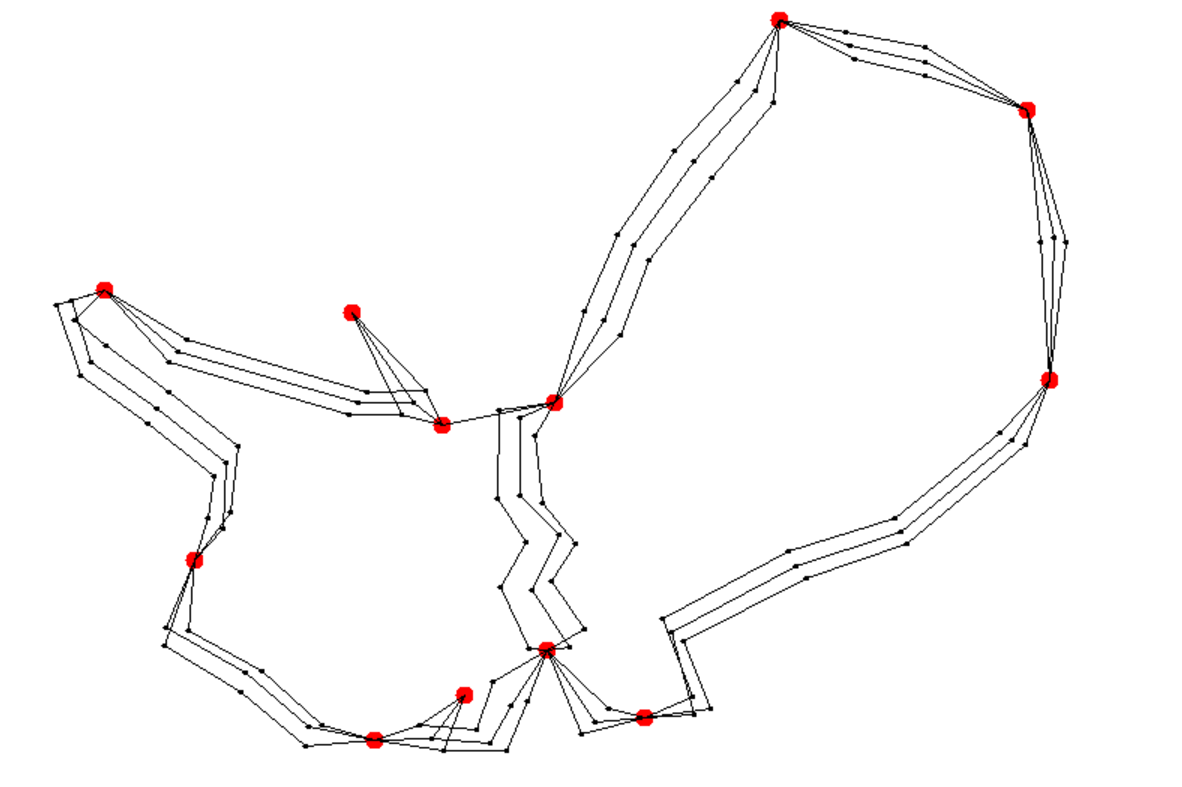
\includegraphics[scale=0.5]{bilder/graphfertig}\label{fig_dortmundmap}
}\\
\caption[Dortmunder MetroMap]{Dortmunder MetroMap [http://www.urbanrail.net/eu/de/do/dortmund-map.png]}
\label{fig_dortmundmap}
\end{figure}
Um das Problem der Ausreißer besser in den Griff zu bekommen und dennoch wieder mehr Topologie in dem Graphen zu bringen, ist es besser eine gänzlich neue Kraft der Abstoßenden und Anziehenden hinzuzufügen. Eine Kraft die nur sicherstellt, dass die Topologie des Graphen beibehalten wird. Das bedeutet die Knoten dürfen sich nicht zu weit von ihrer ursprünglichen Position entfernen. Die Kraft sollte stärker wirken, je weiter die Knoten von ihrer Startposition entfernt sind. Ähnlich der anziehenden Kraft zwischen zwei Knoten, die bereits vorhanden ist. Es müssen sich demnach alle Knoten ihre Startposition merken und stets mit ihrer momentanen Position vergleichen. Hat man diese beiden Informationen, so kann eine weitere anziehende Kraft hinzugefügt werden, welche mit diesen beiden Positionen arbeitet. Das Vorgehen dabei ist relativ simpel. Wird die anziehende Kraft so modifiziert, dass der zweite Knoten nicht mehr ein Knoten ist, sondern die ursprüngliche Position $p^{0}$ des ersten Knotens. So würde es nun eine anziehende Kraft von einem Knoten zu seiner Startposition geben. Diese Kraft muss natürlich auch jede Iteration auf jedem Knoten wirken und genau wie bei der ursprünglichen anziehenden Kraft, dem Vektor des Knotens, welcher die Richtung der Bewegung bestimmt hinzugefügt werden. Dem Algorithmus aus 3.1 wird demnach eine neue anziehende Kraft hinzugefügt, welche im Algorithmus 4.1 durch Zeile 3-6 veranschaulicht wird. Sie ist sehr ähnlich der anziehenden Kraft, nur dass der zweite Knoten durch die ursprüngliche Position $p^{0}$ ersetzt wird. \\
 


Es existieren nun jedoch wieder zu viele anziehende Kräfte, sodass die abstoßende Kraft in Relevanz zu schwach wirkt und die Knoten sich wieder näher zueinander hinziehen als sie sollten. Um das Problem der Ausreißer weitestgehend zu verhindern, wird die abstoßende Kraft nicht erhöht, sondern die beiden anziehenden Kräfte verringert. Experimentell hat sich bewährt, dass eine Schwächung der anziehenden Kraft zwischen benachbarten Knoten von etwa 20\% und eine Schwächung von 50\% der haltenden Kraft, die einen Knoten an ihre ursprüngliche Position hält, die schönsten Layouts bringt, die sich am besten dem Problem angepasst haben. \\

\begin{figure}[t]
	\centering
	\subfigure[deutlich vergrößerter Abstand zwischen den Knoten, der Verlauf wurde jedoch beibehalten]
	{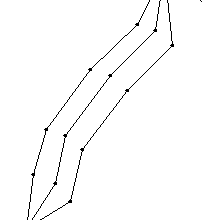
\includegraphics[scale=1.0]{bilder/abstandseile}\label{fig_planar1}
	}
	\hspace{1.0cm}%
	\subfigure[Der Graph mit den modellierten Leiterseilen]
	{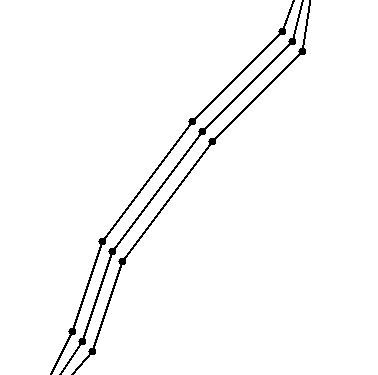
\includegraphics[scale=0.5]{bilder/knotenplacement}\label{fig_planar2}
	}
	\\
	\caption[Vergleich der Leiterseile]{Modellierung der Leiterseile}
	\label{fig_testbild2}
\end{figure}


Auf der Abbildung 4.6 ist das Endergebnis  meiner Arbeit zu sehen. Fast alle Knoten haben einen guten Abstand zueinander, welches auch in Abbildung 4.7 dargestellt wird.  Die Verbindungen sind noch sehr ähnlich ihrem ursprünglichen geographischen Verlauf. Es ist kein Problem zu erkennen, wo die umgangenen Hindernisse sich befanden. Drei Ausreißer sind noch zu sehen, welche sich jedoch nur sehr schwer entfernen lassen. Die Parallelität zwischen den Leiterseilen ist sehr gut zu sehen. Es ist nun möglich bei jeder Verbindung die Anzahl der Leiterseile direkt der Zeichnung zu entnehmen.

\section{Weitere Ansätze zur Verbesserung des Layouts}
\label{Kapitel_4_-_Unterkapitel_4}

Um eine noch bessere Sichtbarkeit der Parallelität zu schaffen, wurden eine weitere Kraft hinzugefügt. Diese Kraft verändert nicht nur die Parallelität der Leiterseile, sondern hat auch einen positiven Einfluss auf die Knoten, die in direkter Verbindung mit den größeren unbeweglichen Städten stehen.
